\documentclass[11pt, a4paper]{article}

\usepackage[top=1 in, bottom = 1 in, left = 1 in, right = 1 in ]{geometry}

\usepackage{amsmath, amssymb, amsfonts}
\usepackage{enumerate}
\usepackage{multirow}
\usepackage{hhline}
\usepackage{array}
\usepackage{longtable}
\usepackage{graphicx}

\title{\textbf{QUESTIONS}}

\author{}
\date{}

\begin{document}

\maketitle

\begin{enumerate}

%01

	\item The following data relate to the life(in hours) of 15 samples of 6 electric bulbs each, drawn at intervals of one hour from a production process. Draw the $\overline{x}$ and $R$ charts and comment.
	
	\begin{table}[h]
	\def\arraystretch{1.5}
	
	\begin{center}

	\begin{tabular}{|c||>{\centering}m{1.5cm}>{\centering}m{1.5cm}>{\centering}m{1.5cm}>{\centering}m{1.5cm}>{\centering}m{1.5cm}>{\centering\arraybackslash}m{1.5cm}|}
	\hline
	Sample No. & \multicolumn{6}{c|}{Life-time (in hours)}	\\
	\hline
	1 & 620 & 687 & 666 & 769 & 839 & 686 \\
	
	2 & 501 & 585 & 524 & 585 & 655 & 668 \\
	
	3 & 673 & 701 & 636 & 567 & 622 & 660 \\
	
	4 & 646 & 626 & 572 & 628 & 632 & 743 \\
	
	5 & 494 & 984 & 659 & 643 & 660 & 640 \\
	
	6 & 634 & 755 & 625 & 582 & 685 & 555 \\
	
	7 & 619 & 710 & 664 & 693 & 773 & 534 \\
	
	8 & 631 & 723 & 614 & 535 & 551 & 570 \\
	
	9 & 482 & 791 & 533 & 612 & 497 & 499 \\
	
	10 & 706 & 524 & 626 & 503 & 662 & 754 \\
	
	11 & 530 & 432 & 379 & 690 & 724 & 536 \\
	
	12 & 485 & 497 & 608 & 393 & 648 & 729 \\
	
	13 & 585 & 535 & 762 & 588 & 625 & 737 \\
	
	14 & 462 & 490 & 635 & 587 & 554 & 673 \\
	
	15 & 722 & 608 & 665 & 587 & 531 & 705 \\
	
	\hline
	
	\end{tabular}
	\end{center}
	
	\end{table}
	
	
	
	
	
	
	
	
	
	
	
%02

	\item A machine is set to deliver the packets of a given weight. Ten samples of size five each were examined and the following results were obtained :
	
	\begin{table}[h]
	\def\arraystretch{1.5}
	
	\begin{center}
	\begin{tabular}{|c|cccccccccc|}
	
	\hline
	
	Sample no. & 1 & 2 & 3 & 4 & 5 & 6 & 7 & 8 & 9 & 10 \\
	
	
	Mean & 43 & 49 & 37 & 44 & 45 & 37 & 51 & 46 & 43 & 47 \\
	
	Range & 5 & 6 & 5 & 7 & 7 & 4 & 8 & 6 & 4 & 6 \\
	
	\hline
	
	\end{tabular}
	\end{center}
	
	\end{table}
	
	Calculate the values for the central line and the control limits for the mean chart and range chart. Comment on the state of control.
	
	
	
	
\newpage





%03
	\item Construct a control chart for mean and the range for the following data on the basis of fuses, samples of 5 being taken every hour(each set of 5 has been arranged in ascending order of magnitude). Comment on whether the production seems to be under contorl, assuming that these are the first data :
	
	\begin{table}[h]
	\def\arraystretch{1.5}
	
	\begin{center}
	\begin{tabular}{|cccccccccccc|}
	
	\hline
	
	42 & 42 & 19 & 36 & 42 & 51 & 60 & 18 & 15 & 69 & 64 & 61 \\
	
	65 & 45 & 24 & 54 & 51 & 74 & 60 & 20 & 30 & 109 & 90 & 78 \\
	
	75 & 68 & 80 & 69 & 57 & 75 & 72 & 27 & 39 & 113 & 93 & 94 \\
	
	78 & 72 & 81 & 77 & 59 & 78 & 95 & 42 & 62 & 118 & 109 & 109 \\
	
	87 & 90 & 81 & 84 & 78 & 132 & 138 & 60 & 84 & 153 & 112 & 136 \\
	
	\hline
	
	\end{tabular}
	\end{center}
	
	\end{table}
	
	
	
	
	
	
%04
	\item The fill volume of soft-drink beverage bottles is an important quality characteristic. The volume is measured (approximately) by placing a gauge over the crown and comparing the height of the liquid in the neck of the bottle against a coded scale. On this scale, a reading of zero corresponds to the correct fill height. Fifteen samples of size n = 10 have been analyzed, and the fill heights are shown in following table :
	
	\begin{table}[h]
	\def\arraystretch{1.5}
	
	\begin{center}
	\begin{tabular}{|c||cccccccccc|}
	
	\hline
	
	Sample Number & $x_1$ & $x_2$ & $x_3$ & $x_4$ & $x_5$ & $x_6$ & $x_7$ & $x_8$ & $x_9$ & $x_{10}$ \\
	
	\hline
	
	1 & 2.5 & 0.5 & 2.0 & $-1.0$ & 1.0 & $-1.0$ & 0.5 & 1.5 & 0.5 & $-1.5$ \\
	
	2 & 0.0 & 0.0 & 0.5 & 1.0 & 1.5 & 1.0 & $-1.0$ & 1.0 & 1.5 & $-1.0$ \\
	
	3 & 1.5 & 1.0 & 1.0 & $-1.0$ & 0.0 & $-1.5$ & $-1.0$ & $-1.0$ & 1.0 & $-1.0$ \\
	
	4 & 0.0 & 0.5 & $-2.0$ & 0.0 & $-1.0$ & 1.5 & $-1.5$ & 0.0 & $-2.0$ & $-1.5$ \\
	
	5 & 0.0 & 0.0 & 0.0 & $-0.5$ & 0.5 & 1.0 & $-0.5$ & $-0.5$ & 0.0 & 0.0 \\
	
	6 & 1.0 & $-0.5$ & 0.0 & 0.0 & 0.0 & 0.5 & $-1.0$ & 1.0 & $-2.0$ & 1.0 \\
	
	7 & 1.0 & $-1.0$ & $-1.0$ & $-1.0$ & 0.0 & 1.5 & 0.0 & 1.0 & 0.0 & 0.0 \\
	
	8 & 0.0 & $-1.5$ & $-0.5$ & 1.5 & 0.0 & 0.0 & 0.0 & $-1.0$ & 0.5 & $-0.5$ \\
	
	9 & $-2.0$ & $-1.5$ & 1.5 & 1.5 & 0.0 & 0.0 & 0.5 & 1.0 & 0.0 & 1.0 \\
	
	10 & $-0.5$ & 3.5 & 0.0 & $-1.0$ & $-1.5$ & $-1.5$ & $-1.0$ & $-1.0$ & 1.0 & 0.5 \\
	
	11 & 0.0 & 1.5 & 0.0 & 0.0 & 2.0 & $-1.5$ & 0.5 & $-0.5$ & 2.0 & $-1.0$ \\
	
	12 & 0.0 & $-2.0$ & $-0.5$ & 0.0 & $-0.5$ & 2.0 & 1.5 & 0.0 & 0.5 & $-1.0$ \\
	
	13 & $-1.0$ & $-0.5$ & $-0.5$ & $-1.0$ & 0.0 & 0.5 & 0.5 & $-1.5$ & $-1.0$ & $-1.0$ \\
	
	14 & 0.5 & 1.0 & $-1.0$ & $-0.5$ & $-2.0$ & $-1.0$ & $-1.5$ & 0.0 & 1.5 & 1.5 \\
	
	15 & 1.0 & 0.0 & 1.5 & 1.5 & 1.0 & $-1.0$ & 0.0 & 1.0 & $-2.0$ & $-1.5$ \\
	
	\hline
	
	
	
	\end{tabular}
	\end{center}
	
	\end{table}
	
	Evaluate the control limits for $\overline{x}$-chart and $s$-chart on this process and comment on the state of control.
	
	
	
	
	
	
\newpage





%05
	\item A high-voltage power supply should have a nominal output voltage of 350 V. A sample of four units is selected each day and tested for process-control purposes. The data shown the following table give the difference between the observed reading on each unit and the nominal voltage times ten; that is $x_i = (\text{observed voltage on unit } i - 350)10$.
	
	\begin{table}[h]
	\def\arraystretch{1.5}
	
	\begin{center}
	\begin{tabular}{|>{\centering}m{3cm}||>{\centering}m{1.5cm}>{\centering}m{1.5cm}>{\centering}m{1.5cm}>{\centering\arraybackslash}m{1.5cm}|}
	
	\hline
	
	Sample Number & $x_1$ & $x_2$ & $x_3$ & $x_4$ \\
	
	\hline
	
	1 & 6  & 9  & 10  & 15 \\

	2 & 10 &  4 &  6  & 11 \\

	3 & 7  & 8 &  10 &  5 \\

	4 & 8  & 9 &  6  & 13 \\

	5 & 9  & 10 &  7  & 13 \\

	6 & 12 &  11  & 10  & 10 \\

	7 & 16 &  10 & 8 &  9 \\

	8 & 7  & 5 &  10 &  4 \\

	9 & 9  & 7 &  8  & 12 \\

	10 & 15 &  16  & 10  & 13 \\

	11 & 8  & 12  & 14  & 16 \\

	12 & 6  & 13 &  9  & 11 \\

	13 & 16 &  9  & 13  & 15 \\

	14 & 7  & 13  & 10  & 12 \\

	15 & 11 &  7  & 10  & 16 \\

	16 & 15 &  10  & 11  & 14 \\

	17 & 9  & 8  & 12  & 10 \\

	18 & 15 &  7  & 10  & 11 \\

	19 & 8  & 6 &  9  & 12 \\
	
	20 & 13 &  14  & 11  & 15 \\
	
	\hline

	
	\end{tabular}
	\end{center}
	
	\end{table}

Set up $\overline{x}$-chart and $s$-chart on this process. Is the process in statistical control ?






%06
	\item Following are the figures for the number of defectives in 22 lots, each containing 2000 rubber belts :
	
	425, 430, 216, 341, 225, 322, 280, 306, 337, 305, 356, 402, 216, 264, 126, 409, 193, 326, 280, 389, 451, 420.
	
	Drawing the control chart for fraction defective, plot the points on it. Comment on the state of control of the process.
	
	
	Also calculate the control limits of the control chart for percent defective.
	
	
	
	
	
	
	
	
	
\newpage








%07
	\item The data in the following table give the number of nonconforming bearing and seal assemblies in samples of size 100. Construct a fraction nonconforming control chart for these data. If any points plot out of control, assume that assignable causes can be found and determine the revised control limits.
	
	
	\begin{table}[h]
	\def\arraystretch{1.5}
	
	\begin{center}
	\begin{tabular}{|>{\centering}m{3cm}|>{\centering}m{4cm}||>{\centering}m{3cm}|>{\centering\arraybackslash}m{4cm}|}
	
	\hline
	
	Sample Number & Number of Nonconforming Assemblies & Sample Number & Number of Nonconforming Assemblies \\
	
	\hline
	
	1  & 7 & 11 &  6 \\
	
	2  & 4 & 12  & 15 \\ 
	
	3  & 1 & 13 &  0 \\  
	
	4  & 3 & 14 &  9 \\  
	
	5  & 6 & 15 &  5 \\  
	
	6  & 8 & 16 &  1 \\  
	
	7  & 10 & 17 &  4 \\ 
	
	8  & 5 & 18 &  5 \\  
	
	9  & 2 & 19 &  7 \\
	
	10 &  7 & 20  & 12 \\
		
	 	
 	
 	\hline

	\end{tabular}
	\end{center}
	\end{table}
	
	
	
	
	
	
	
	
	
%08

	\item The following data give the number of defectives in 10 independent samples of varying sizes from a production process :
	
	\begin{table}[h]
	\def\arraystretch{1.5}
	
	\begin{center}
	\begin{tabular}{|>{\centering}m{3cm}||>{\centering}m{0.7cm}>{\centering}m{0.7cm}>{\centering}m{0.7cm}>{\centering}m{0.7cm}>{\centering}m{0.7cm}>{\centering}m{0.7cm}>{\centering}m{0.7cm}>{\centering}m{0.7cm}>{\centering}m{0.7cm}>{\centering\arraybackslash}m{0.7cm}|}
	
	
	\hline
	
	Sample Number & 1 & 2 & 3 & 4 & 5 & 6 & 7 & 8 & 9 & 10 \\
	
	\hline
	
	Sample size & 2000 & 1500 & 1400 & 1350 & 1250 & 1760 & 1875 & 1955 & 3125 & 1575 \\
	
	\hline
	
	No. of defectives & 425 & 430 & 216 & 341 & 225 & 322 & 280 & 306 & 337 & 305 \\
	
	\hline
	
	
	\end{tabular}
	\end{center}
	
	\end{table}


Construct suitable control chart for fraction defective and comment on it.














%09
	\item 20 samples each of size 10 were inspected. The number of defectives detected in each of them is given below :
	
	\begin{table}[h]
	\def\arraystretch{1.5}
	
	\begin{center}
	\begin{tabular}{|>{\centering}m{3cm}||>{\centering}m{0.5cm}>{\centering}m{0.5cm}>{\centering}m{0.5cm}>{\centering}m{0.5cm}>{\centering}m{0.5cm}>{\centering}m{0.5cm}>{\centering}m{0.5cm}>{\centering}m{0.5cm}>{\centering}m{0.5cm}>{\centering\arraybackslash}m{0.5cm}|}
	
	\hline
	
	Sample Number & 1 & 2 & 3 & 4 & 5 & 6 & 7 & 8 & 9 & 10 \\
	
	\hline
	
	No. of defectives & 0 & 1 & 0 & 3 & 9 & 2 & 0 & 7 & 0 & 1 \\\hline\hline
	
	Sample Number & 11 & 12 & 13 & 14 & 15 & 16 & 17 & 18 & 19 & 20 \\
	
	\hline
	
	No. of defectives & 1 & 0 & 0 & 3 & 1 & 0 & 0 & 2 & 1 & 0 \\
	
	\hline
	
	\end{tabular}
	\end{center}
	
	\end{table}

Construct the \textit{number of defectives} chart and establish quality standard for the future.







\newpage






%10
	\item In welding of seams, there are defects included pinholes, cracks, cold taps, etc. A record was made of the number of defects found in one seam each hour and is given below.
	
	\begin{table}[h]
	\def\arraystretch{1.5}
	
	\begin{center}
	\begin{tabular}{|>{\centering}m{3cm}|>{\centering}m{3cm}|>{\centering\arraybackslash}m{2cm}|}
	
	\hline
	
	1.12.2005 & 8 A.M. & 2 \\
	
	& 9 A.M. & 4 \\
	
	& 10 A.M. & 7 \\
	
	& 11 A.M. & 3 \\
	
	& 12 P.M. & 1 \\
	
	& 1 P.M. & 4 \\
	
	& 2 P.M. & 8 \\
	
	& 3 P.M. & 9 \\
	
	\hline
	
	2.12.2005 & 8 A.M. & 5 \\
	
	& 9 A.M. & 3 \\
	
	& 10 A.M. & 7 \\
	
	& 11 A.M. & 11 \\
	
	& 12 P.M. & 6 \\
	
	& 1 P.M. & 4 \\
	
	& 2 P.M. & 9 \\
	
	& 3 P.M. & 9 \\
	
	\hline

	3.12.2005 & 8 A.M. & 6 \\
	
	& 9 A.M. & 4 \\
	
	& 10 A.M. & 3 \\
	
	& 11 A.M. & 9 \\
	
	& 12 P.M. & 7 \\
	
	& 1 P.M. & 4 \\
	
	& 2 P.M. & 7 \\
	
	& 3 P.M. & 12 \\
	
	\hline
	
	
	
	\end{tabular}
	\end{center}
	
	\end{table}
	
	Construct the control chart for number of defects and give your comments.
	
	
	
	
	
	
	
\newpage
	
	
	
	
	
%11
	\item The number of workmanship nonconformities observed in the final inspection of disk-drive assemblies has been tabulated as shown in the following table. Does the process appear to be in control?
	

	\begin{table}[h]
	\def\arraystretch{1.5}
	
	\begin{center}
	\begin{tabular}{|>{\centering}m{2cm}|>{\centering}m{6cm}|>{\centering\arraybackslash}m{6cm}|}
	
	
	\hline
	
	Day & Number of Assemblies Inspected & Total Number of Imperfections \\
	
	\hline
	
	1 & 2 & 10 \\
	
	2 & 4 & 30 \\
	
	3 & 2 & 18 \\
	
	4 & 1 & 10 \\
	
	5 & 3 & 20 \\
	
	6 & 4 & 24 \\
	
	7 & 2 & 15 \\
	
	8 & 4 & 26 \\
	
	9 & 3 & 21 \\
	
	10 & 1 & 8 \\
	
	\hline
	\end{tabular}
	\end{center}
	
	\end{table}
	
	
	
	
	
	
	
	
	
	
	
	
	
	
	
	
	
	
	
	
%12
	\item For a lot consisting of 2200 items, a sample of size 225 is taken. If it contains 14 or less defectives, the lot is accepted otherwise rejected. Plot the $OC$, $ATI$ and $AOQ$ curves.
	
	
	
	
	
	
	
	
	
	
%13
	\item In a single sampling inspection plan for attributes with $n = 52$ and $c = 2$, draw the $OC$ curve and comment. It it known that the lot is large.
	
	
	
\vspace{50pt}
	
\begin{figure}[h]
\centering
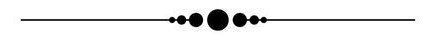
\includegraphics[scale=0.4]{end}
\end{figure}	
	
	
	
	
	
	
	
	
	
\end{enumerate}
\end{document}